\begin{figure*}[t]
\centering
\setlength{\figwidth}{0.10\textwidth}
\begin{tabular}{c c c c c c}
  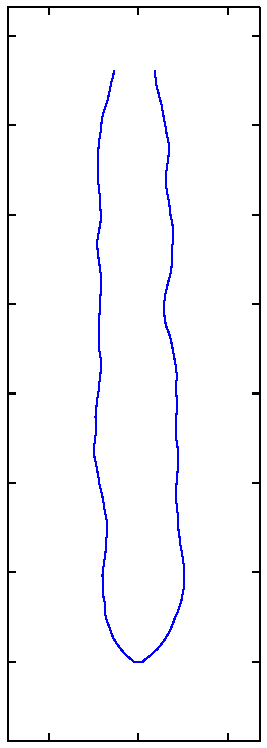
\includegraphics[width=\figwidth]{\figpath/path_points} &
  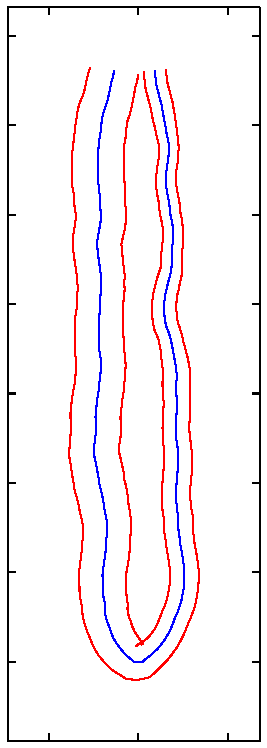
\includegraphics[width=\figwidth]{\figpath/edge_points} &
  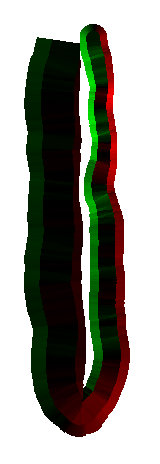
\includegraphics[width=\figwidth]{\figpath/u_gt}
  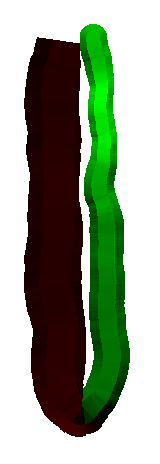
\includegraphics[width=\figwidth]{\figpath/v_gt} &
  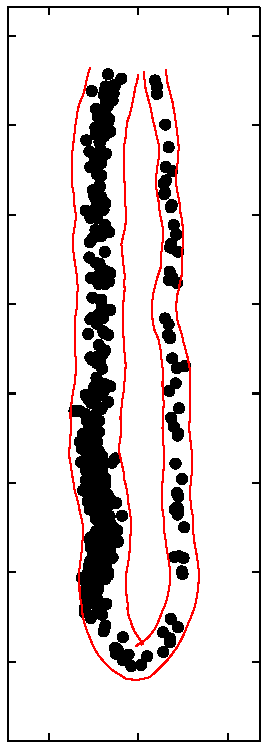
\includegraphics[width=\figwidth]{\figpath/cells_positions} &
  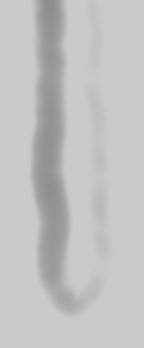
\includegraphics[width=\figwidth]{\figpath/clean} &
  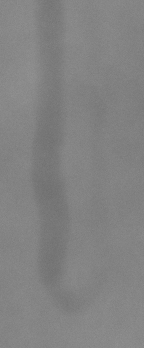
\includegraphics[width=\figwidth]{\figpath/fake_cap} \\
  (a) & (b) & (c) & (d) & (e) & (f)
\end{tabular}
%
\caption{Image synthesis process: (a) path of the vessel centre; (b) edges of the venous and arterial limb; (c) horizontal and vertical flow fields, respectively; (d) blood cell positions along the vessel centre; (e) synthetic image, before adding noise artefacts; (f) final synthetic image. For the flow fields in (c), hue indicates the direction of flow over the sequence (green is right/down, red is left/up) and intensity is proportional to flow rate (black indicates zero flow).}
\label{fig_image_generation}
\end{figure*}
